\documentclass [xcolor=dvipsnames] {beamer}

\usepackage[utf8] {inputenc}
\usepackage{ngerman}
\usepackage{graphicx}
\usepackage{pgfpages}
\usepackage[printwatermark]{xwatermark}
\usepackage{tikz}

\setbeameroption{show notes on second screen}

%\usetheme {Antibes}
%\usetheme{PaloAlto}
%\usetheme{Montpellier}
\usecolortheme [named=Maroon] {structure}

\title {\sc Neulandeuphonie}
\author {Jakob Schade, Jeremy Kolbe, Karl Engelhardt, Markus Schmidl, Martin Heckel}

%draft watermark
\newsavebox\watermark
\savebox\watermark{\tikz[color=gray,opacity=0.3]\node{DRAFT};}
\newwatermark*[allpages,angle=45,scale=6,xpos=-20,ypos=15]{\usebox\watermark}

\begin{document}

%titlepage
\begin{frame}
	\titlepage
\end{frame}

%toc
\begin{frame}
	\tableofcontents
\end{frame}

%wer
\section{Wer?}
\begin{frame}
	\begin{center}
		{\Huge Wer?}
	\end{center}
\end{frame}
\begin{frame}
	\setbeamertemplate{caption}{{\color{Maroon}JHOst 2015:} \insertcaption}
	\begin{figure}
		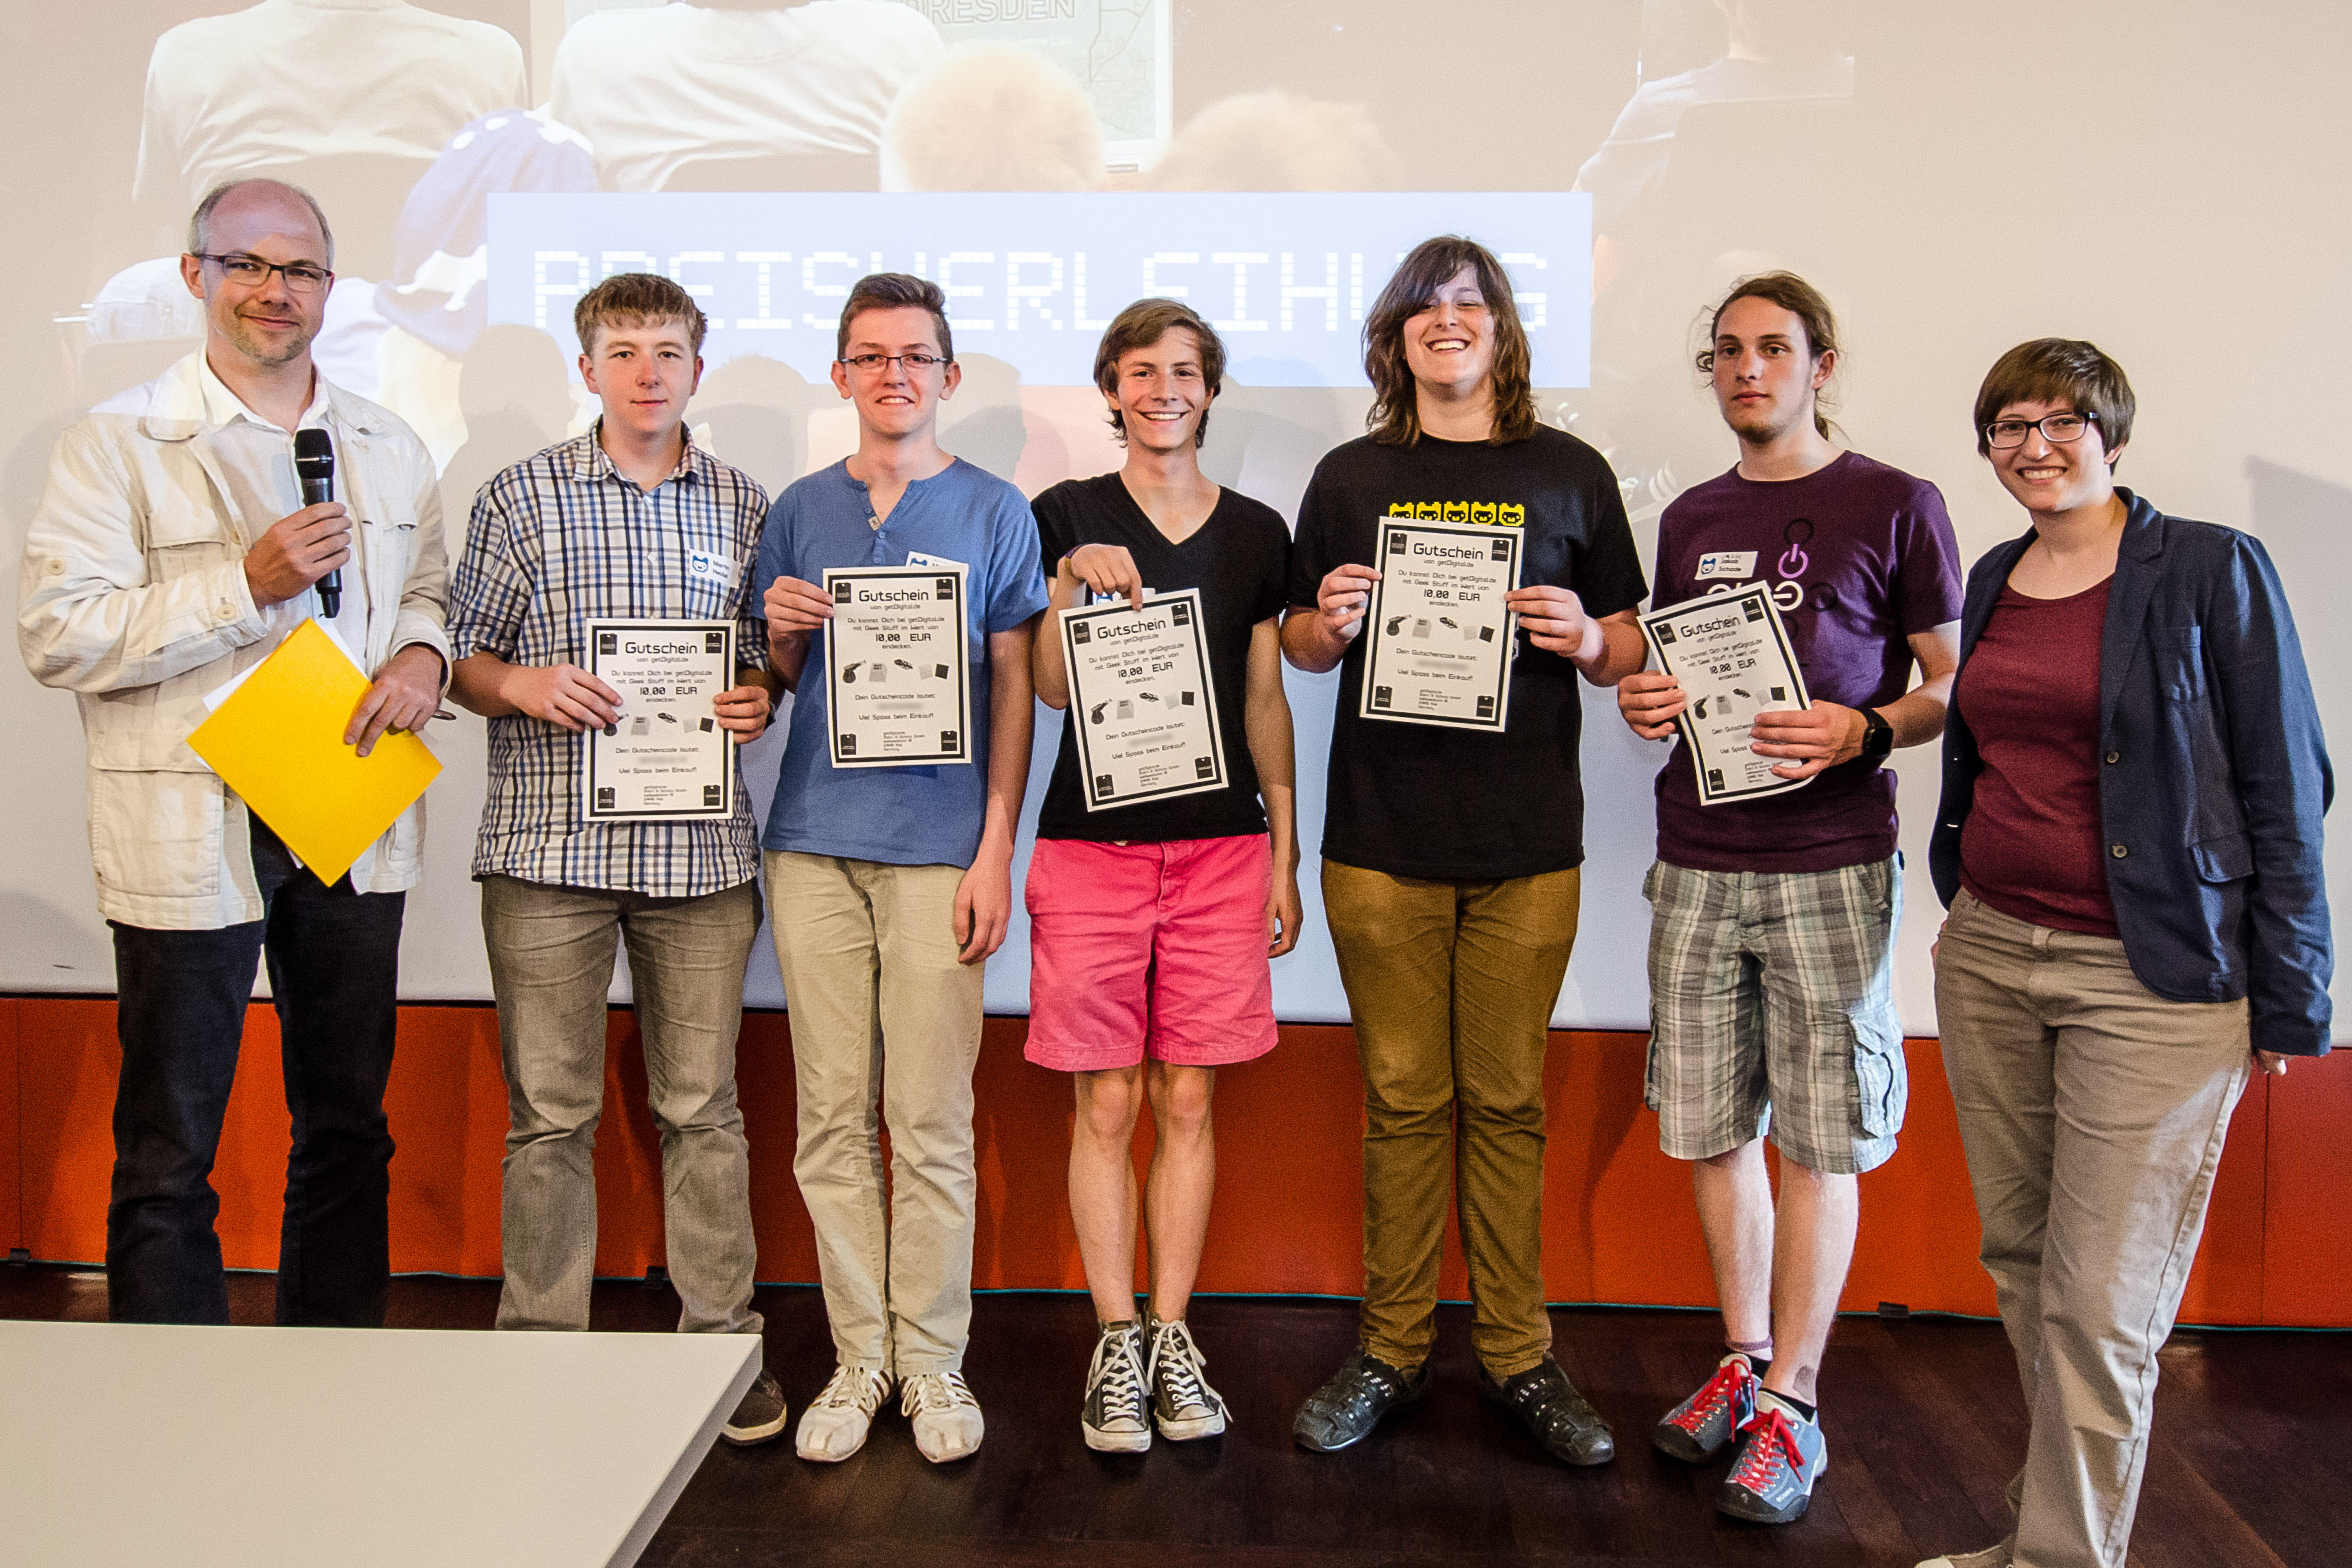
\includegraphics[width=10cm]{jhost2015abschluss}
		\caption{CC BY-SA 2.0 Jugend hackt, Foto: Steffen Haas}
	\end{figure}
\end{frame}

%neulandeuphonie?
\section{Neulandeuphonie?}
\subsection{Das Problem}
\begin{frame}
	\frametitle{\sc Das Problem}
	\begin{center}
		{\Huge Zensur}
	\end{center}
\end{frame}
\note[itemize]
{
	\item Great Firewall of China
}

\subsection{Das Ziel}
\subsubsection{Schaffen von Aufmerksamkeit}
\begin{frame}
	\only<1>{\frametitle{\sc Das Ziel}}
	\begin{center}
		\only<2>
		{
			{\Huge Wie?}
		}
		\only<3>
		{
			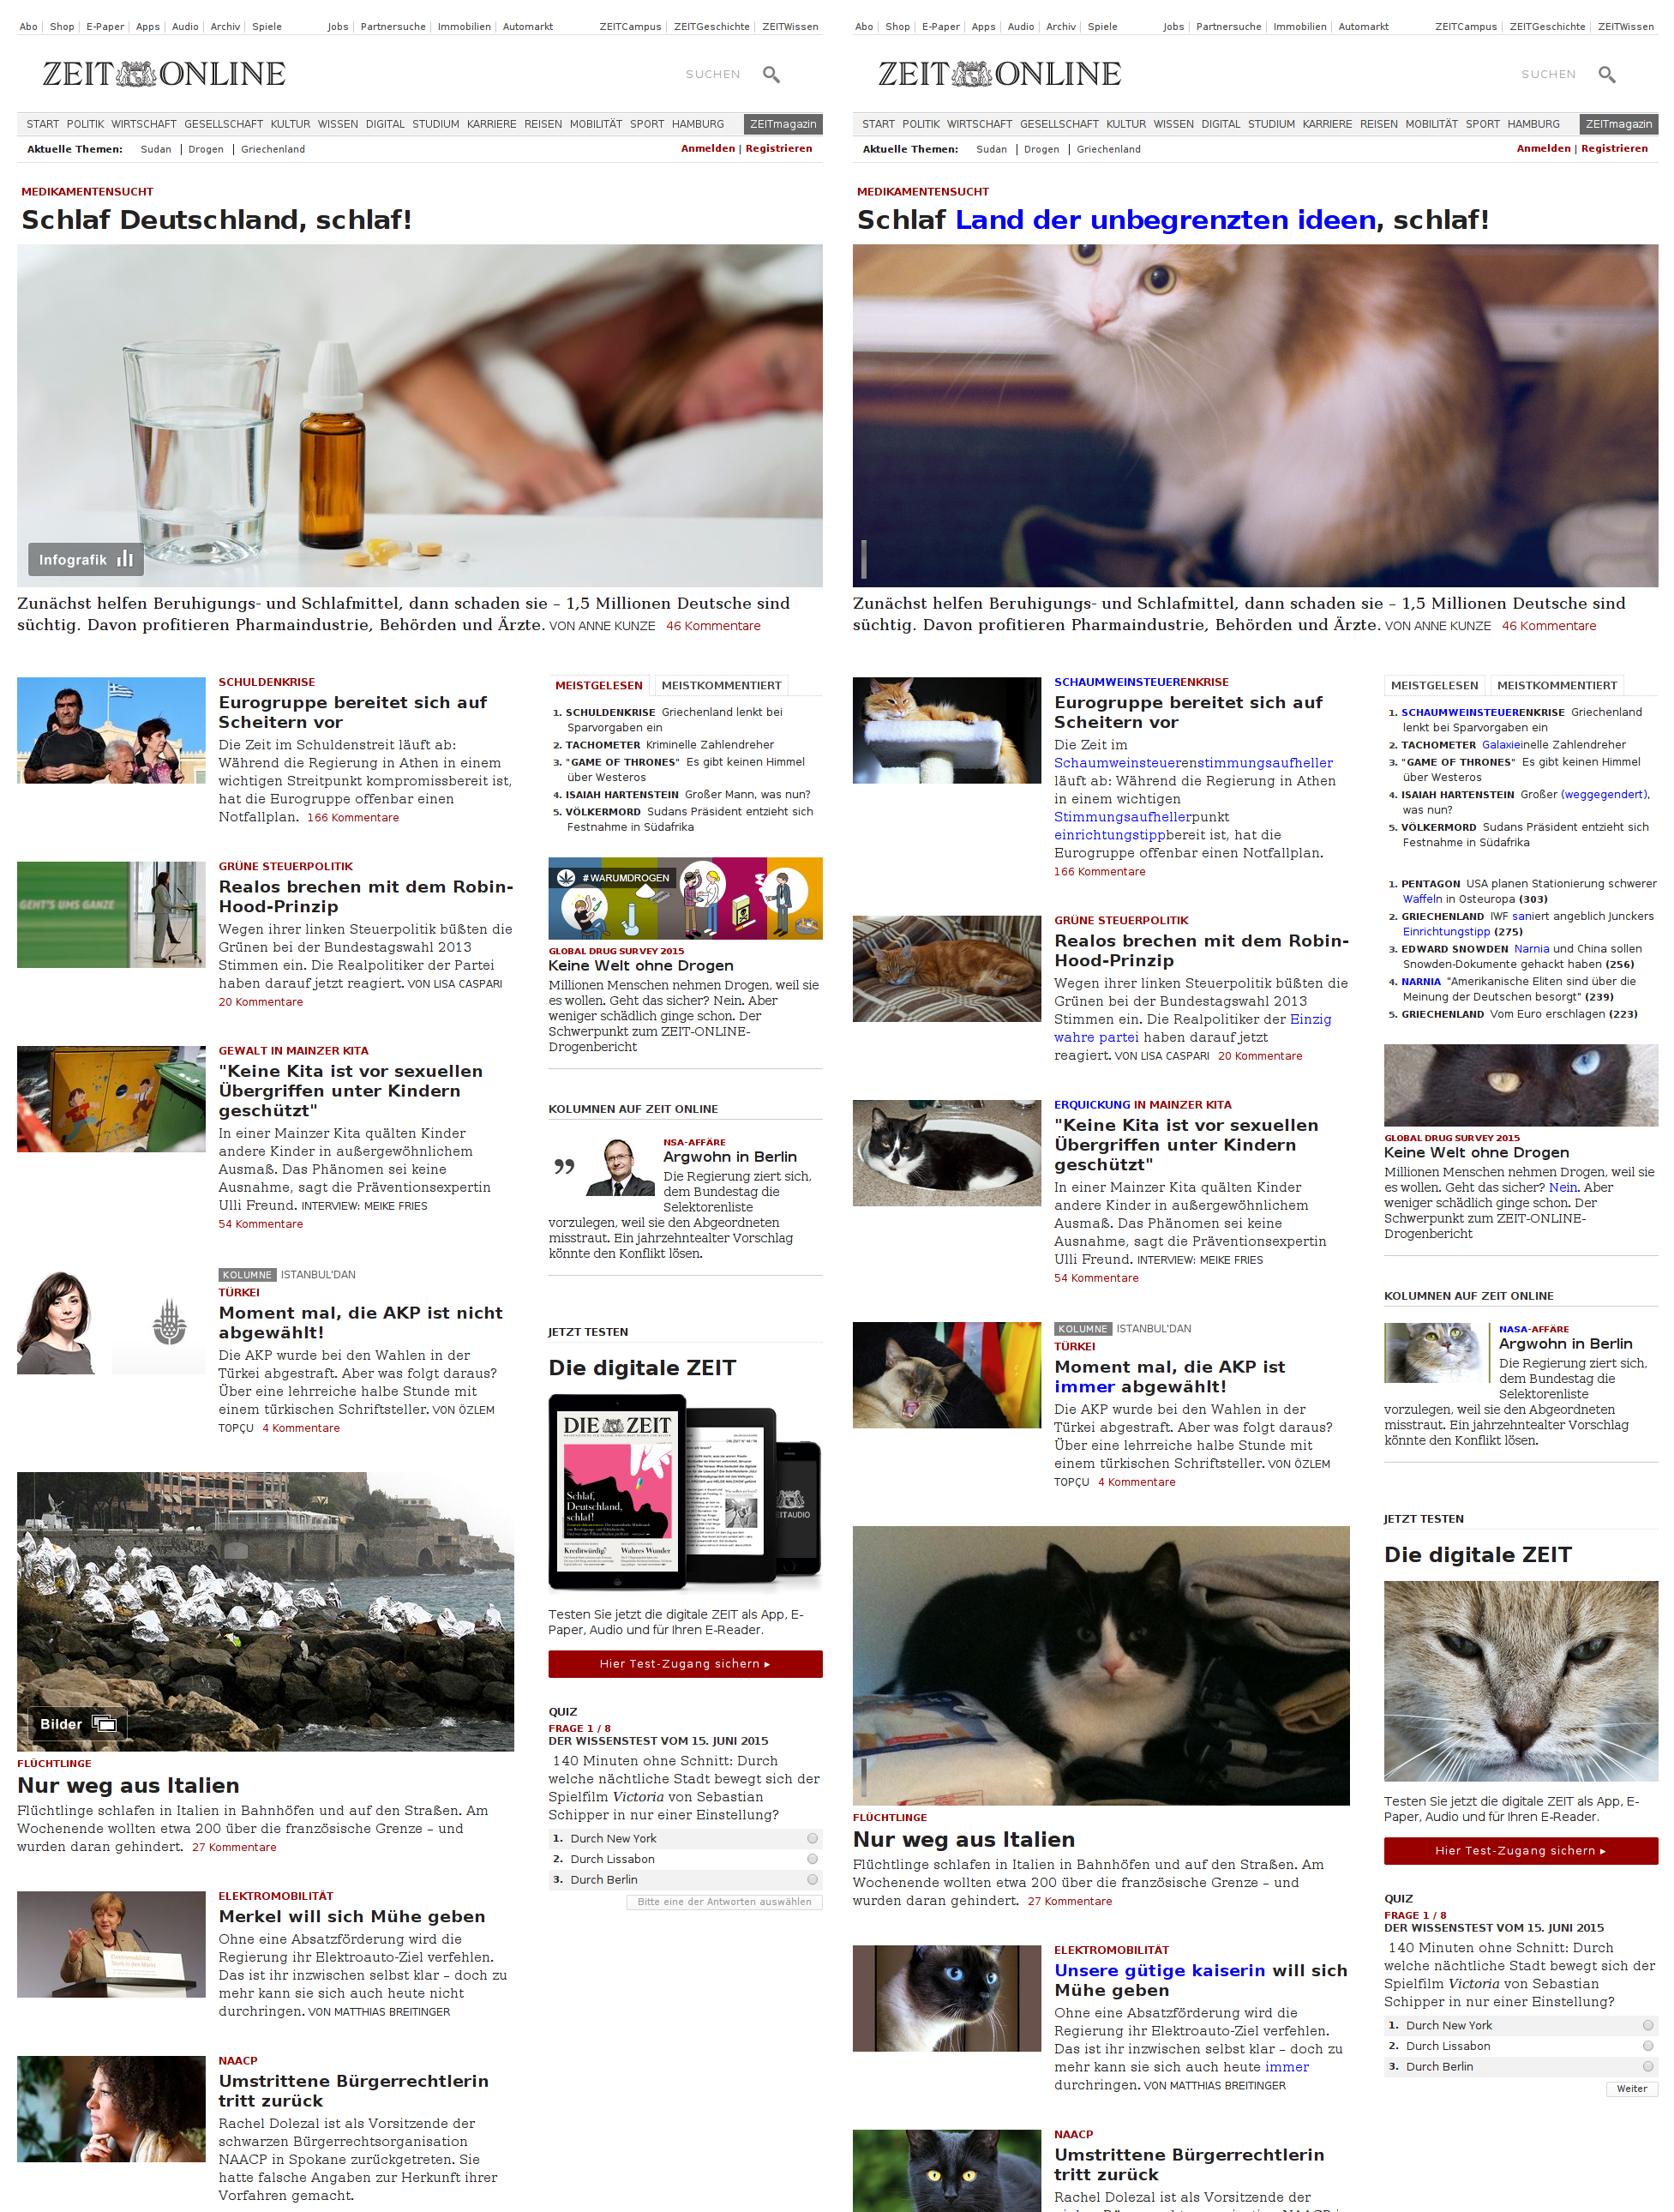
\includegraphics[width=10cm]{combined}
		}
		\only<1>
		{
			Schaffunng von Aufmerksamkeit auf Zensur mit Zensur
		}
	\end{center}
\end{frame}
\note[itemize]
{
	\item Bildzensur
	\item Wortzensur
}

\subsubsection{Unser Motto}
\begin{frame}
	\frametitle{\sc Motto}
	\begin{center}
		\only<1>
		{
			{\bf Die Welt steht vor dem Abgrund!}\\ \ \\ Für diejenigen unter uns, die das absolut nicht verarbeiten können, gibt es nun Neulandeuphonie!
		}
		\only<2>
		{
			Neulandeuphonie is a censoring proxy that replaces bad words with good ones and all images with images of cats (everybody loves cats). This change in site demonstrates how easy it is to manipulte website and how people need to live in counries which are known for blocking (e.g. the majority of China).
		}
	\end{center}
\end{frame}

%methoden
\section{Methoden}
\subsection{Wortzensur}
\begin{frame}
	\frametitle{\sc Wortzensur}
	\begin{center}
		{\it Wörter werden ausgetauscht und Blau eingefärbt}
		\ \\
	\end{center}
	\begin{tabular}{l|l}
		originales Wort & mit Neulandeuphonie\\
		\hline
		(Angela) Merkel & Mutti\\
		& Unsere gütige Kaiserin\\
		& Unsere gütige Kaiserin in Gottes Gnaden\\
		Pfefferspray & Sprühsahne\\
		illegal & legal\\
		Bombe & Torte\\
		Waffe & Waffel\\
		National Security Agency & freundliche Anti-Terror-Organisation\\
		Bayern & Weißwurstland\\
		explode* & flan*\\
		& fantas*
	\end{tabular}
\end{frame}

\subsection{Bildzensur}
\begin{frame}
	{\sc Bildzensur}
	\begin{center}
		\only<1>
		{
			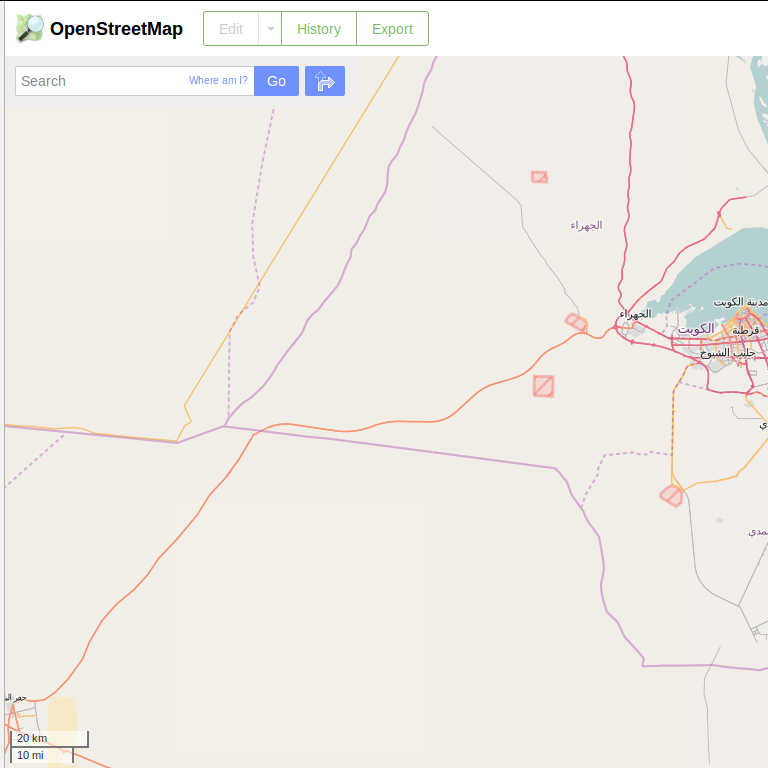
\includegraphics[width=10cm]{osm-1}
		}
		\only<2>
		{
			{\Large zu}
		}
		\only<3>
		{
			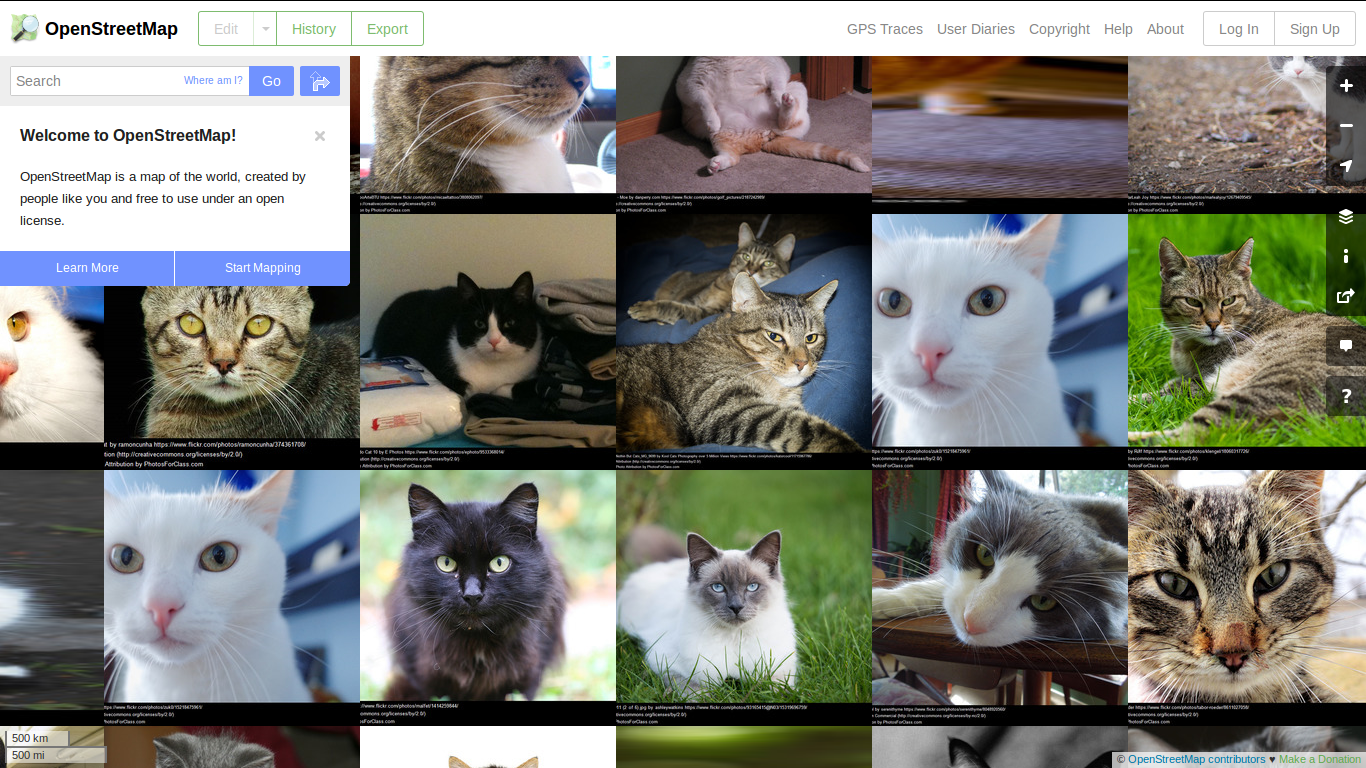
\includegraphics[width=10cm]{osm-mod-1}
		}
	\end{center}
\end{frame}

%technische Umsetzung
\section{Technische Umsetzung}
\begin{frame}
	{\sc Allgemein}
	\begin{itemize}
		\item Python: 216 LoC
		\item Regex
		\item libmproxy
	\end{itemize}
\end{frame}
\note
{
	{\Large TODO: Add technical fuu}
	
}
\begin{frame}
	{\sc Teile}
	\begin{itemize}
		\item proxy.py
		\item proxy_functions.py
	\end{itemize}
\end{frame}
\note
{
	{\Large Die proxy.py macht den allegemeinen aufbau, aber kein ersetzen. die proxy_functions macht das ersetzen, kann leicht erweitert/ersetzt werden. je nach content type wird bild oder text ersetzt}
	
}
\subsection{Technisches Problem und dessen Lösung}
\begin{frame}
	\frametitle{\sc Technisches Problem}
	\begin{center}
		\begin{itemize}
			\item LANGSAM
		\end{itemize}
	\end{center}
\end{frame}
\note
{
	{\Large jedes HTML-Tag: paar hundert "`Regular Expressions"', 3-6 Sekunden pro seite}
	
}
\begin{frame}
	\frametitle{\sc Die Lösung}
	\begin{center}
		{\Large NeulandeuphonieJS}
	\end{center}
	\begin{itemize}
		\item Chromeplugin
		\item weitaus bessere Perfomance
		\item zur Zeit nur Textaustausch
		\item kann deaktiviert werden
	\end{itemize}
\end{frame}
\note
{
	{\Large fällt kaum auf, zeigt 1 sec den original text an, ersetzt nur, bilder austausch noch nicht gebaut}
	
}
%interessiert
\begin{frame}
	\frametitle{\sc Interessiert?}
	\begin{center}
		{\bf https://github.com/Jugendhackt/neulandeuphonie}
	\end{center}
\end{frame}
\note
{
	{\Large TODO: add notice for help}
	\\
	Still from MB21
}

%endblatt
\begin{frame}
	\titlepage
\end{frame}

\end{document}
